\renewcommand{\figurename}{Rys.}

\chapter{Badania eksperymentalne i~interpretacja wyników}
\label{cha:test}

\fontsize{14}{15}\selectfont
%----------------------------------------------------------

Silne ukrwienie dłoni umożliwia dokonywanie pomiarów pulsoksymetrem na wszystkich końcówkach palców bez znacznego wpływu na osiągane wyniki 
pomiarów,~np.~\ref{rys:Dlon}.
\begin{figure}[!ht]
	\centerline{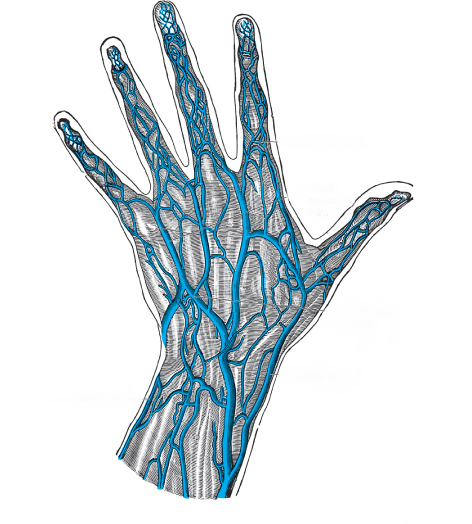
\includegraphics[scale = 0.56]{graphic/Dlon}}
	\caption{Układ naczyń krwionośnych dłoni i~palców człowieka}
	\label{rys:Dlon}
	~\\	
	(źródło: Na podstawie \cite{SzGa11})
\end{figure}

W~trakcie mierzenia pulsu zwraca się uwagę na 6 charakterystycznych cech tętna bazując na kształcie krzywej pletyzmograficznej~\cite{SzGa11}.

\noindent \textbf{Częstotliwość} - (liczba wyczuwanych uderzeń w~ciągu minuty), której wartości prawidłowe zależą głównie od wieku. W~czasie badania na uwadze 
należy mieć, że nie należy badać tętna po wysiłku fizycznym (po dużym wysiłku fizycznym częstotliwość może nawet przekraczać 200 uderzeń/min.) lub w~stanie 
silnych przeżyć emocjonalnych. Tętno może być częste (\emph{pulsus frequens}) lub rzadkie (\emph{pulsus rarus}). Przeciętna częstotliwość tętna waha się w~zależności 
od wieku i~wynosi około:
\begin{itemize}
	\item u~płodu: 110-150 [1/min]
	\item u~niemowląt: 130 [1/min]
	\item u~dzieci: 100 [1/min]
	\item u~młodzieży: 85 [1/min]
	\item u~dorosłych: 70 [1/min]
	\item u~ludzi starszych: 60 [1/min]
\end{itemize}
\noindent \textbf{Miarowość} - tętno jest miarowe (\emph{pulsus regularis}) jeśli wszystkie uderzenia wykazują jednakową siłę, a~odstępy między nimi są jednakowe, 
w~przeciwnym razie mówimy o~tętnie niemiarowym (\emph{pulsus irregularis}).

\noindent \textbf{Wypełnienie} - określa wysokość fali tętna i~zależy od wypełnienia tętnicy krwią, co z~kolei zależy od rzutu serca. Tętno może być wysokie (duże) 
(\emph{pulsus altus, pulsus magnus}), małe (\emph{pulsus parvus}), nitkowate, równe (\emph{pulsus equalis}), nierówne i~dziwaczne (\emph{pulsus paradoxus}).

\noindent \textbf{Napięcie} - cecha tętna będąca wyrazem ciśnienia tętniczego. Tętno może być twarde (\emph{pulsus durus}), miękkie (\emph{pulsus mollis}) bądź dwubitne.

\noindent \textbf{Chybkość} - zależy od szybkości wypełniania się tętnicy i~zapadania jej światła w~okresie jednego cyklu pracy serca. Zależy od prędkości przepływu krwi 
i~podatności ściany tętnic. Tętno może być chybkie (\emph{pulsus celer}) lub leniwe (\emph{pulsus tardus}).

\noindent \textbf{Symetria} - fizjologicznie tętno powinno być takie samo po lewej i~po prawej stronie ciała.

Średnie tętno spoczynkowe zależy przede wszystkim od wieku i~stopnia wytrenowania,~np.~\ref{rys:TetnoTabela}.
\begin{figure}[ht]
	\centerline{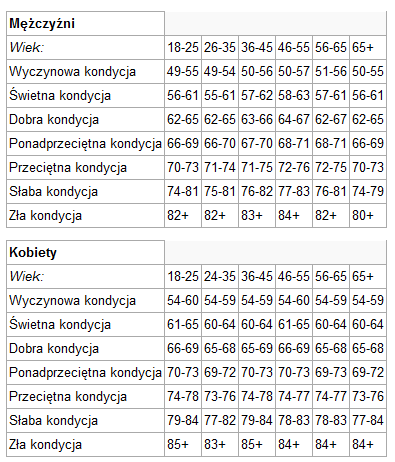
\includegraphics[scale = 1.1]{graphic/TetnoTabela}}
	\caption{Zależność tętna spoczynkowego od wieku, płci i~kondycji organizmu}
	\label{rys:TetnoTabela}
	~\\	
	(źródło: Na podstawie \cite{SzGa11})
\end{figure}


\section{Pomiar częstości akcji serca}
\label{sec:Puls}

Pomiaru tętna, czyli częstości skurczów serca na minutę dokonuje się analizując przebieg krzywej pletyzmograficznej.
Charakterystyczny zmienny przebieg krzywej $PPG$ jest skutkiem zmian objętości naczyń krwionośnych pod wpływem przepływającej krwi pompowanej przez mięsień 
sercowy. Skurcze komór serca zwiększające objętość naczyń tętniczych są widoczne jako lokalne ekstrema krzywej pletyzmograficznej~(rys.~\ref{rys:MAX}).
\begin{figure}[!ht]
	\centerline{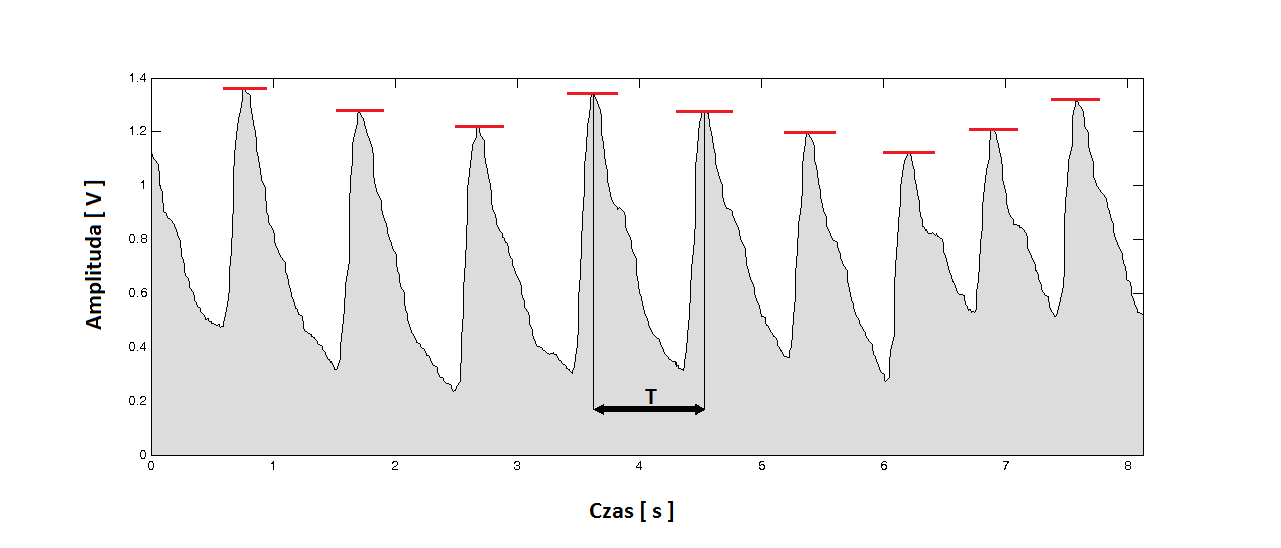
\includegraphics[scale = 0.58]{graphic/MAX}}
	\caption{Moment skurczu komór serca zarejestrowany na przebiegu krzywej pletyzmograficznej $PPG$. Pomiar dokonany zaprojektowanym pulsoksymetrem}
	\label{rys:MAX}
\end{figure}

Praktycznie, chwilowa wartość częstości akcji serca wyznaczana przez pulsoksymetr obliczana jest z~następującej zależności:
\begin{equation}
	BPM = \frac{60}{T}~~[1/min]
\end{equation}
gdzie:\\
$T$ - okres pomiędzy kolejnymi uderzeniami serca w~sekundach.

Poprawności pomiaru zaprojektowanego pulsoksymetru autor dokonał poprzez porównanie uzyskanych wyników z~wynikami komercyjnego ciśnieniomierza typu Hartmann Tensoval Mobil,
wyposażonego w~funkcję pomiaru tętna~(rys.~\ref{rys:tensoval}).
\begin{figure}[!ht]
	\centerline{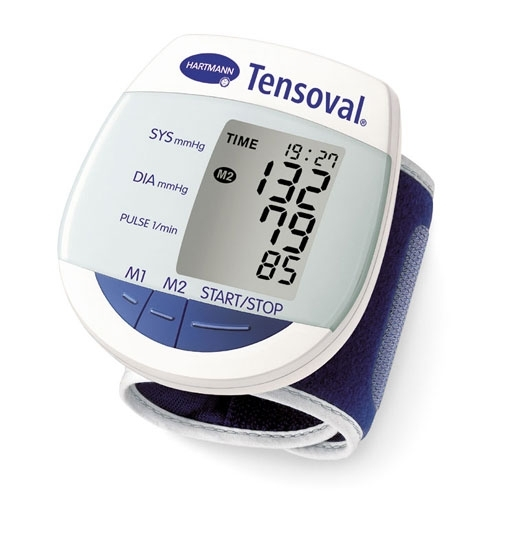
\includegraphics[scale = 0.38]{graphic/tensoval}}
	\caption{Ciśnieniomierz nadgarstkowy Tensoval Mobil firmy Hartmann}
	~\\
	(źródło: http://www.tensoval.pl)
	\label{rys:tensoval}
\end{figure}

Analiza porównawcza ma na celu stwierdzenie poprawności wyników uzyskanych podczas pomiaru tętna przy użyciu zaprojektowanego pulsoksymetru. Urządzenie
umożliwia pomiar chwilowej częstości skurczów komór serca. Punkt odniesienia stanowi wynik pomiaru ciśnieniomierza nadgarstkowego, którego wynik 
określa średnią częstotliwość uderzeń serca w~ciągu trwania pomiaru ciśnienia.

\noindent Wynik pomiaru częstości akcji serca u~pacjenta w~stanie spoczynku przedstawia przebieg na rysunku~\ref{rys:Tetno_D_2}.
\begin{figure}[!h]
	\centerline{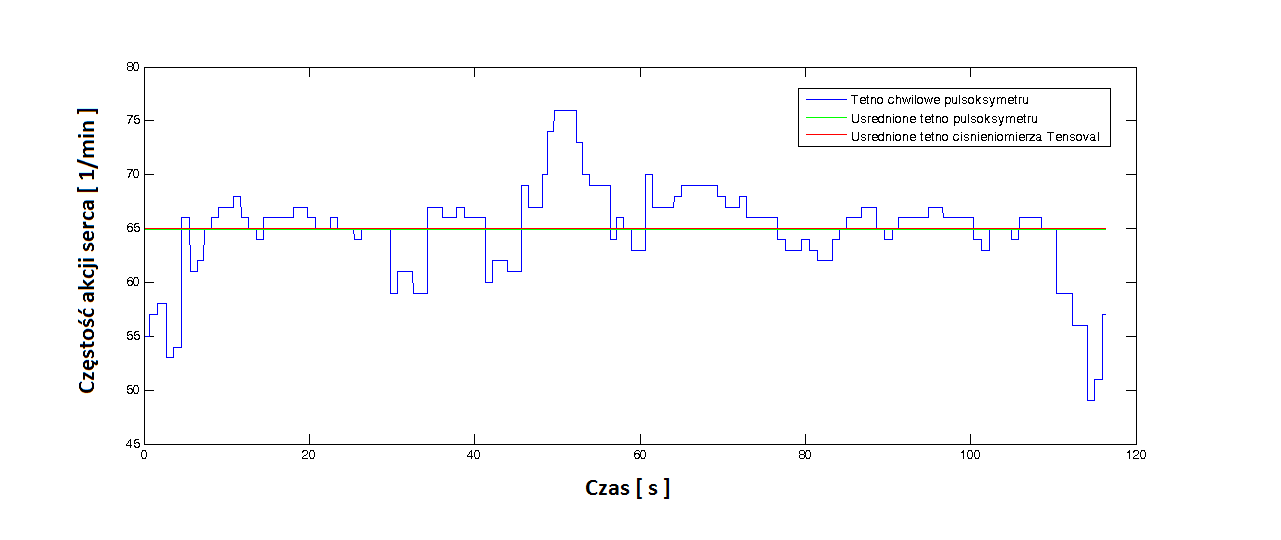
\includegraphics[scale = 0.63]{graphic/Tetno_D_2}}
	\caption{Pomiar chwilowego oraz średniego tętna pacjenta w~stanie spoczynku}
	\label{rys:Tetno_D_2}
\end{figure}

\noindent Chwilowa wartość tętna zawiera się w~zakresie dopuszczalnych wartości dla człowieka zdrowego wynoszącym od 60 do 80 uderzeń na minutę. 
Średnia wartość częstotliwości pulsoksymetru pokrywa się z~wynikiem uzyskanym przy pomocy urządzenia Tensoval.
\noindent Wzmożona praca mięśni organizmu w~trakcie wysiłku fizycznego wymaga dostarczenia większej ilości tlenu do komórek ciała, co skutkuje zwiększeniem
częstotliwości skurczów serca~(rys.~\ref{rys:Tetno_D_1}). 
\begin{figure}[!ht]
	\centerline{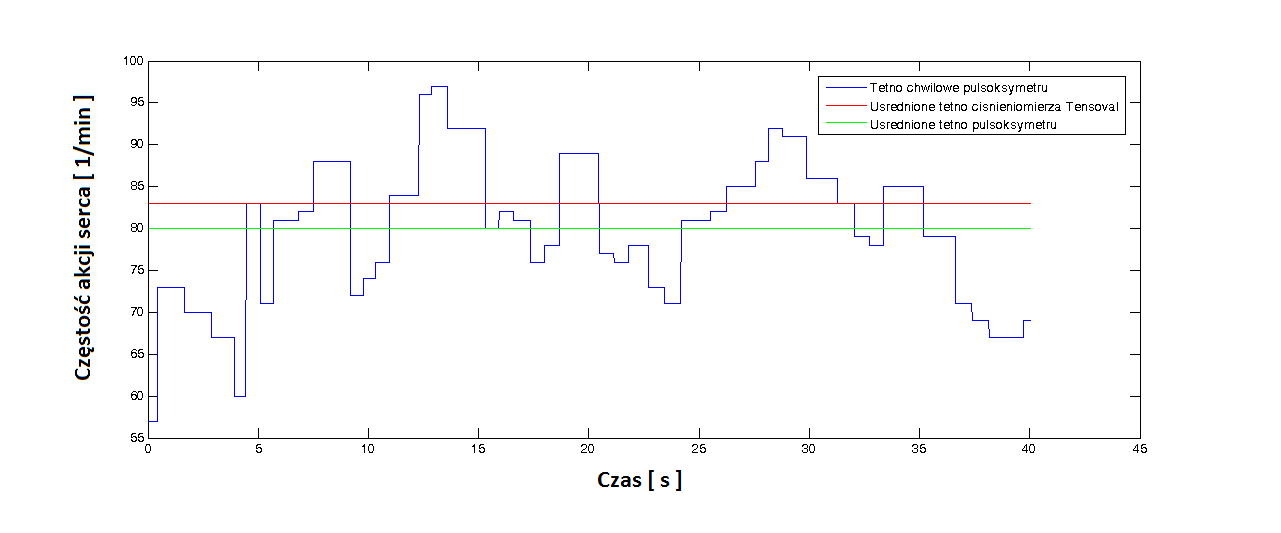
\includegraphics[scale = 0.62]{graphic/Tetno_D_1}}
	\caption{Pomiar chwilowego oraz średniego tętna pacjenta w~trakcie wysiłku fizycznego}
	\label{rys:Tetno_D_1}
\end{figure}

\noindent Podczas weryfikacji poprawności pomiarów pulsoksymetru dokonano serii pomiarów częstości akcji serca u~pacjentów
w różnych przedziałach wiekowych. Wyniki pomiarów przedstawiają przebiegi z~rysunków~\ref{rys:2L}, \ref{rys:25L}, \ref{rys:30L},
\ref{rys:50-60M}, \ref{rys:50-60K} oraz \ref{rys:90L}.
\begin{figure}[!ht]
	\centerline{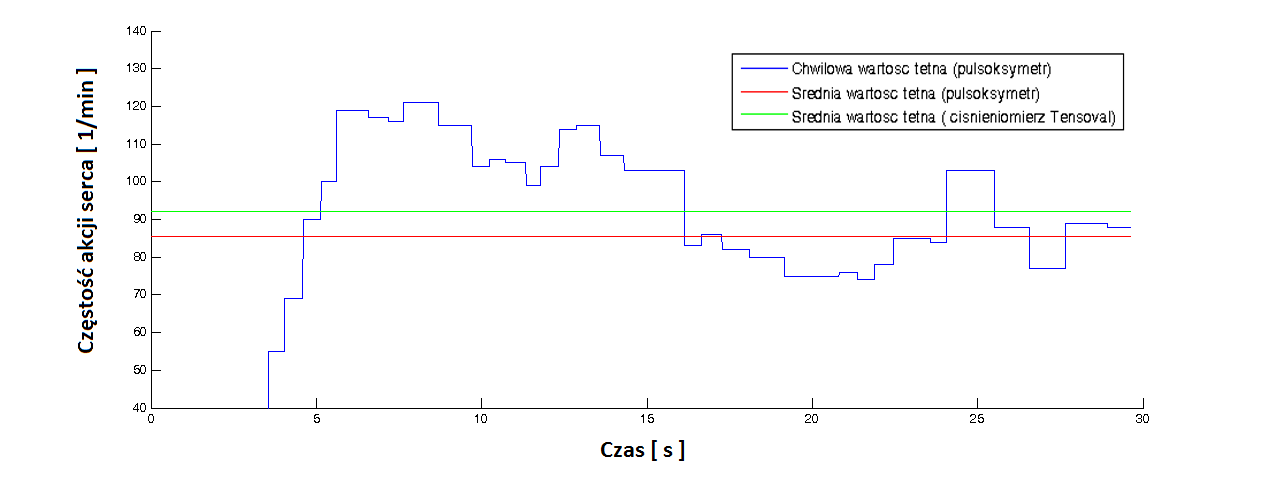
\includegraphics[scale = 0.6]{graphic/2L}}
	\caption{Pomiar chwilowego oraz średniego tętna pacjenta w~wieku 2 lat (chłopiec)}
	\label{rys:2L}
\end{figure}

\noindent Średnia wartość tętna u~dziecka jest zdecydowanie wyższa niż u~młodzieży oraz osób starszych i~zawiera się w~granicach 
80~-~90~[1/min]. 
\begin{figure}[!h]
	\centerline{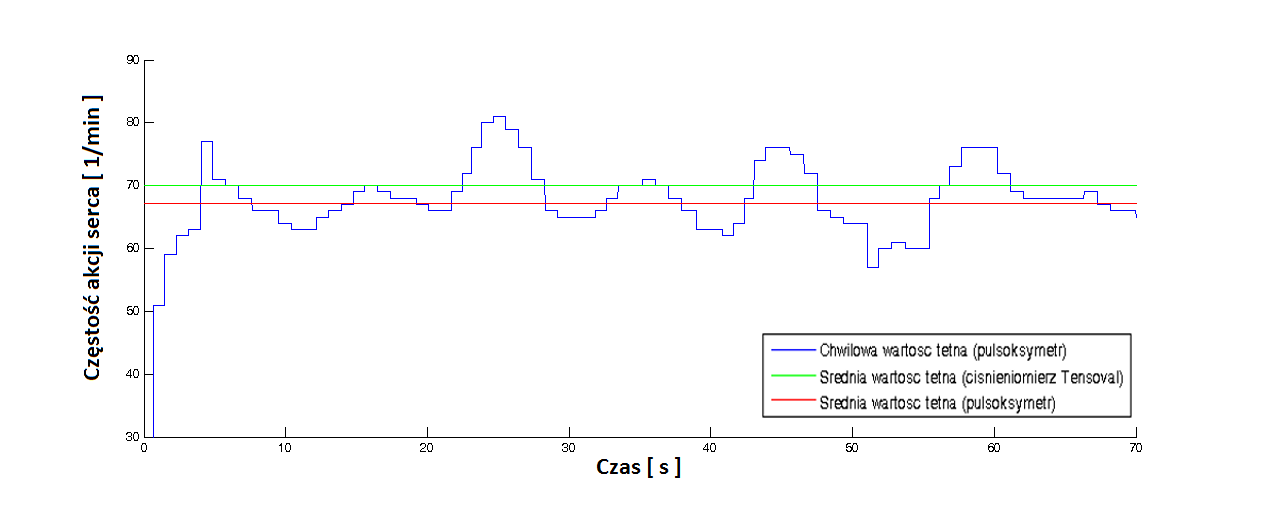
\includegraphics[scale = 0.6]{graphic/25L}}
	\caption{Pomiar chwilowego oraz średniego tętna pacjenta w~wieku 25 lat (mężczyzna)}
	\label{rys:25L}
\end{figure}
\newpage
\begin{figure}[!ht]
	\centerline{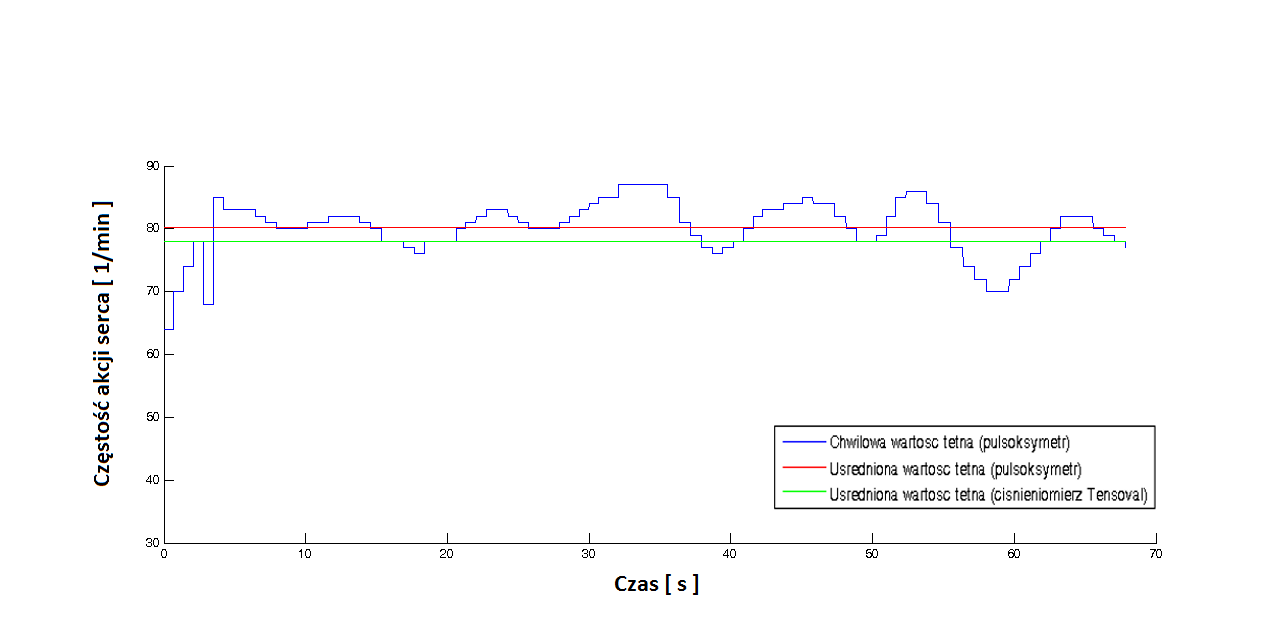
\includegraphics[scale = 0.6]{graphic/30L}}
	\caption{Pomiar chwilowego oraz średniego tętna pacjenta w~wieku 30 lat (mężczyzna)}
	\label{rys:30L}
\end{figure}
\begin{figure}[!hb]
	\centerline{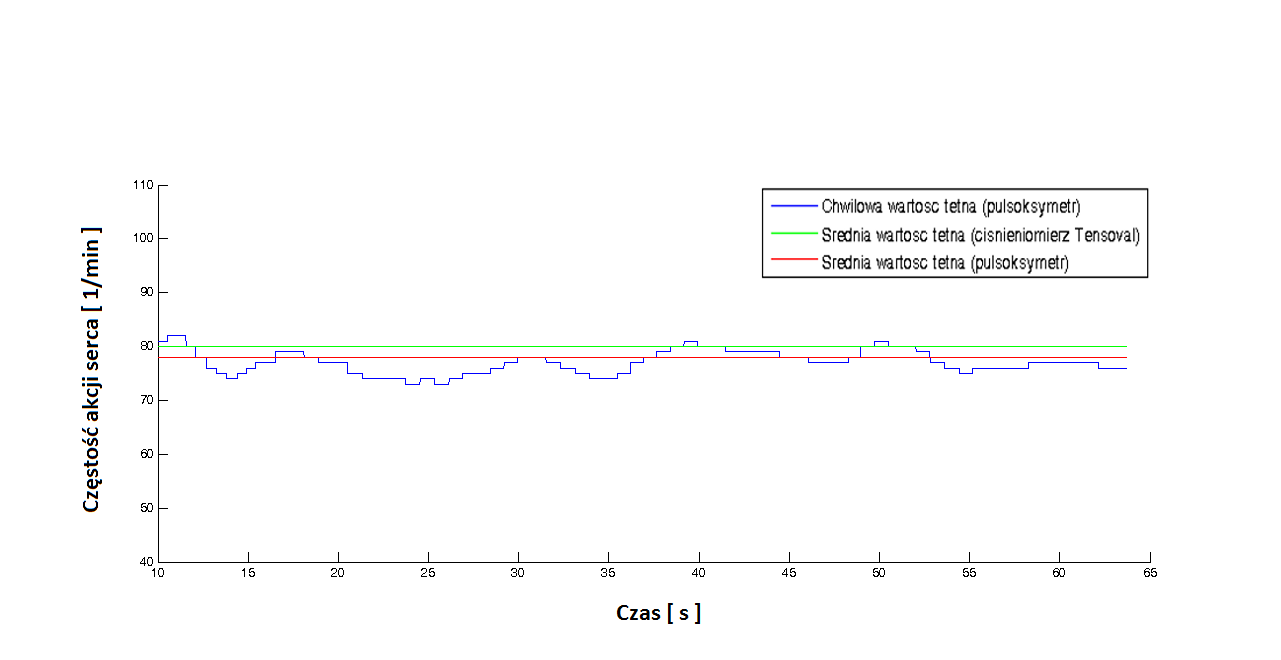
\includegraphics[scale = 0.6]{graphic/50-60M}}
	\caption{Pomiar chwilowego oraz średniego tętna pacjenta w~przedziale wiekowym 50~-~60 lat (mężczyzna)}
	\label{rys:50-60M}
\end{figure}
\newpage
\begin{figure}[!ht]
	\centerline{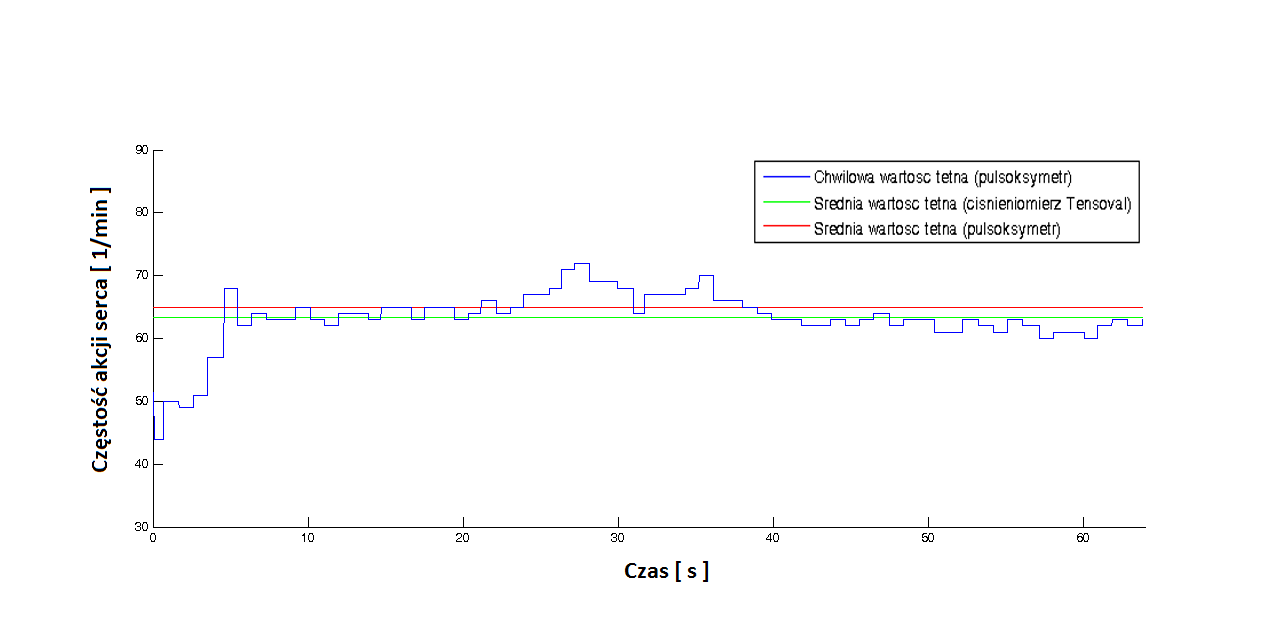
\includegraphics[scale = 0.61]{graphic/50-60K}}
	\caption{Pomiar chwilowego oraz średniego tętna pacjenta w~przedziale wiekowym 50~-~60 lat (kobieta)}
	\label{rys:50-60K}
\end{figure}

\begin{figure}[!hb]
	\centerline{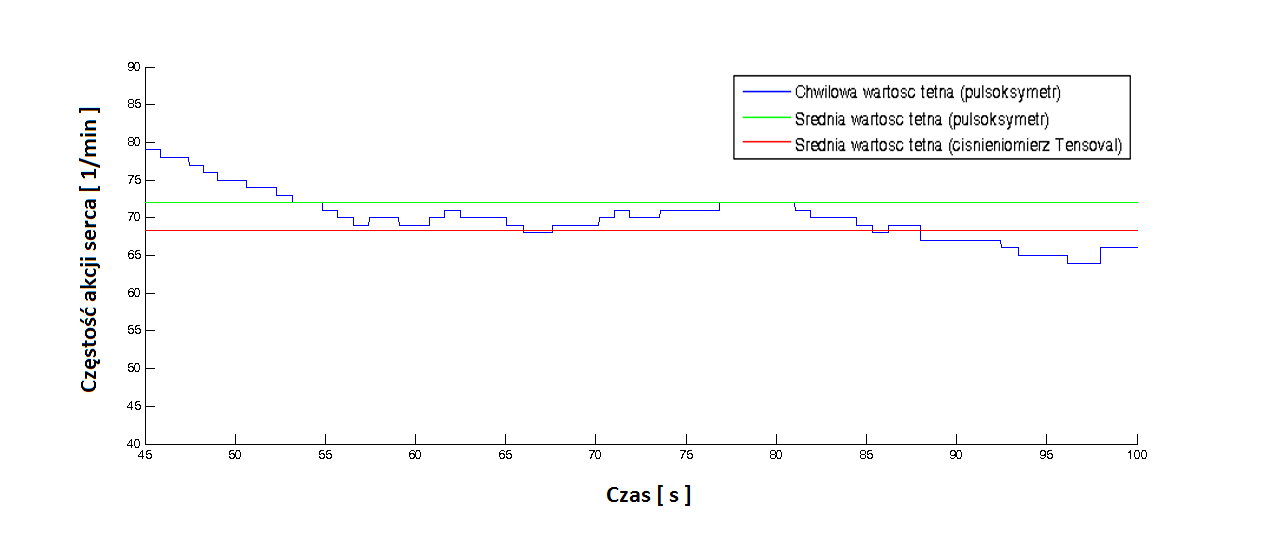
\includegraphics[scale = 0.61]{graphic/90L}}
	\caption{Pomiar chwilowego oraz średniego tętna pacjenta w~wieku 90 lat (kobieta)}
	\label{rys:90L}
\end{figure}
\newpage

Wynik testu dotyczącego powtarzalności uzyskiwanych wyników przedstawiono na rysunku~\ref{rys:proba}.
Przeprowadzone pomiary potwierdzają wpływ wieku i~kondycji pacjenta na osiągane wyniki częstości skurczów serca. Jednocześnie
poprzez analizę porównawczą dowiedziono poprawności pomiarów tętna przy użyciu zaprojektowanego pulsoksymetru.
Odstępności od wyników urządzenia Tensoval spowodowane są umiejscowieniem sondy pomiarowej, metodą pomiaru oraz sposobem
przedstawiania wyników (uśrednianie).
\begin{figure}[!h]
	\centerline{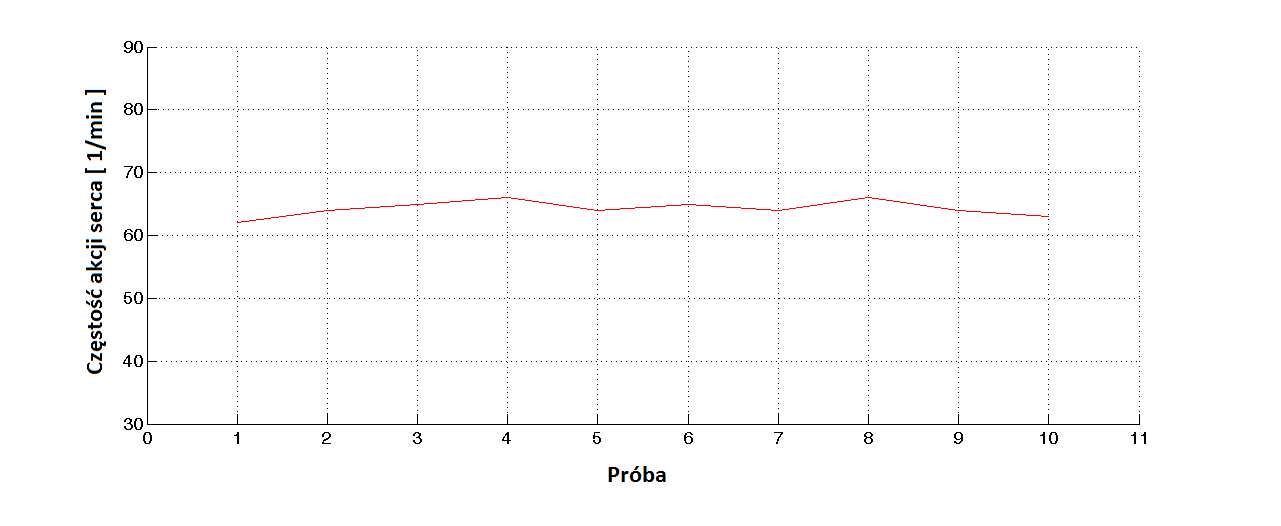
\includegraphics[scale = 0.6]{graphic/proba}}
	\caption{Wartość tętna pacjenta podczas kolejnych prób pomiarowych}
	\label{rys:proba}
\end{figure}

\section{Pomiar wysycenia krwi tętniczej tlenem ($SpO2$)}
\label{sec:Saturacja}

Odmienne właściwości optyczne oksyhemoglobiny oraz hemoglobiny, powodujące różny stopień absorpcji promieniowania przez krew,
powodują detekcję sygnału krzywej pletyzmograficznej o~różnej amplitudzie~(rys.~\ref{rys:PPG1}).
\begin{figure}[!ht]
	\centerline{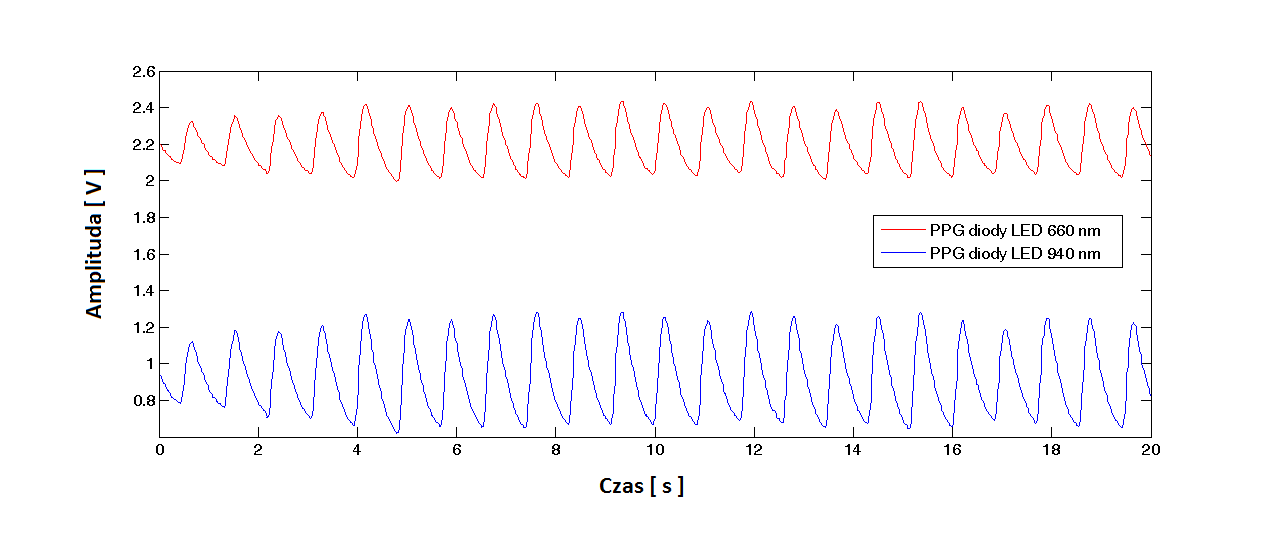
\includegraphics[scale = 0.6]{graphic/PPG1}}
	\caption{Przebieg krzywej PPG dla promieniowania 660~nm oraz 940~nm}
	\label{rys:PPG1}
\end{figure}

Pomiarów wysycenia krwi tętniczej tlenem dokonano metodą wyliczania współczynnika R zależnego od amplitudy sygnału $PPG$ podczas
skurczu i~rozkurczu komór serca~(wzór~\ref{sec:Fotopletyzmografia}). Zaprojektowany pulsoksymetr wykorzystuje następującą zależność 
saturacji krwi w~funkcji współczynnika R~(rys.~\ref{rys:curve}). 
\begin{figure}[!h]
	\centerline{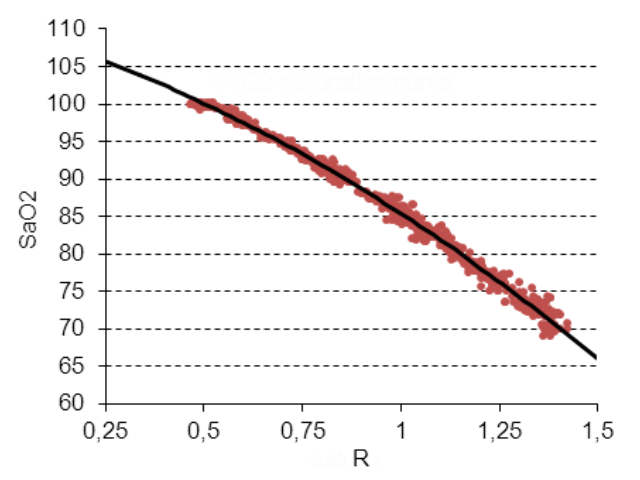
\includegraphics[scale = 0.51]{graphic/curve}}
	\caption{Empiryczna krzywa kalibracji pulsoksymetru}
	\label{rys:curve}
	~\\	
	(źródło: Na podstawie \cite{Katja:2011})
\end{figure}

\noindent Krzywa kalibracji została stworzona na bazie doświadczeń prowadzonych w~laboratorium na próbkach krwi o~różnych stopniach 
natlenowania (in vitro)~\cite{Katja:2011}.

Autor porównał parametry osiągane za pomocą zaprojektowanego urządzenia z~wynikiem komercyjnego pulsoksymetru Respironix Novametrix COSMO, co 
stanowi podstawę do stwierdzenia poprawności funkcjonowania urządzenia~(rys.~\ref{rys:COSMO}).
\begin{figure}[!ht]
	\centerline{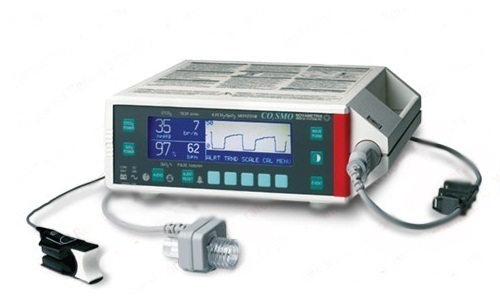
\includegraphics[scale = 0.80]{graphic/COSMO}}
	\caption{Pulsoksymetr szpitalny Respitronix Novametrix COSMO}
	\label{rys:COSMO}
	~\\
	(źródło: http://www.somatechnology.com)
\end{figure}
Poprawny parametr SpO2 zawiera się w~granicach 95\%~–~99\%~\cite{SzGa11}. Pomiar wysycenia krwi tlenem badanego aparatu w~stosunku 
do pomiaru urządzeniem szpitalnym przedstawiono na rysunku~\ref{rys:Saturacja1}.
\begin{figure}[!ht]
	\centerline{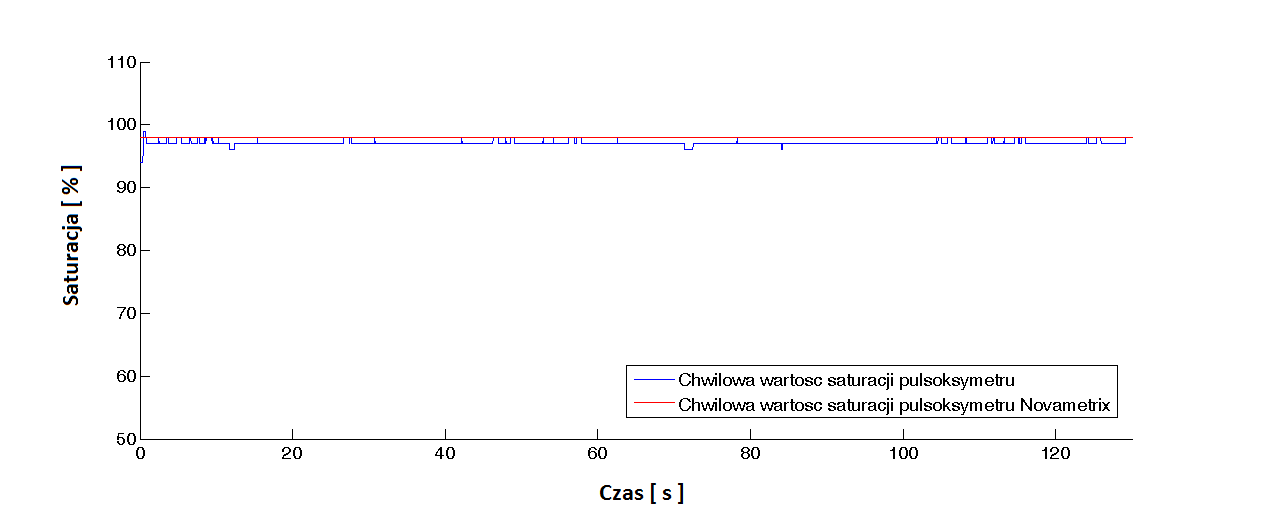
\includegraphics[scale = 0.60]{graphic/Saturacja1}}
	\caption{Zestawienie uzyskanych wyników saturacji przy użyciu dwóch różnych aparatów pomiarowych}
	\label{rys:Saturacja1}
\end{figure}

Uzyskane wyniki wykazują zbieżność pomiarów zaprojektowanego urządzenia z~pomiarem wykonanym aparatami komercyjnymi. Wartości saturacji zdrowego organizmu
oscylują z~niewielką amplitudą wokół wartości 97~\%, mieszczącej się w~dopuszczalnym zakresie.

W~celu stwierdzenia zgodności pomiarów wartości saturacji należy przeprowadzić serię pomiarów na grupie pacjentów o~zróżnicowanym stopniu
natlenowania krwi tętniczej. Zatrucia tlenkiem węgla, długotrwałe palenie tytoniu, anemia, sinica lub terapia tlenowa to główne powody 
zmiany stopnia natlenowania krwi. Trudności z~dostępem do odpowiedniej grupy pacjentów wymuszają przeprowadzenie pomiarów weryfikacyjnych 
na osobach zdrowych. Podczas pomiarów saturacji dokonano zróżnicowania wyników ze względu na wiek badanych osób, np.~\ref{rys:Sat25}, 
\ref{rys:Sat30K}, \ref{rys:Sat30M}, \ref{rys:Sat50M} oraz \ref{rys:Sat90}.\\
\begin{figure}[!h]
	\centerline{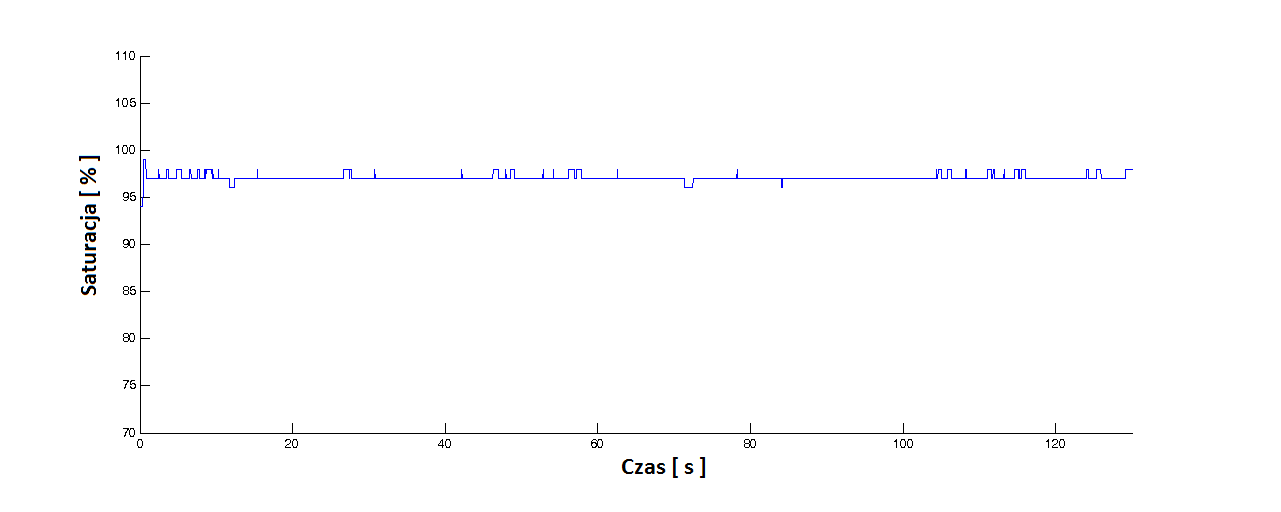
\includegraphics[scale = 0.63]{graphic/Sat25}}
	\caption{Pomiar saturacji chwilowej - pacjent w~wieku 25 lat (mężczyzna)}
	\label{rys:Sat25}
\end{figure}
\newpage
\begin{figure}[!h]
	\centerline{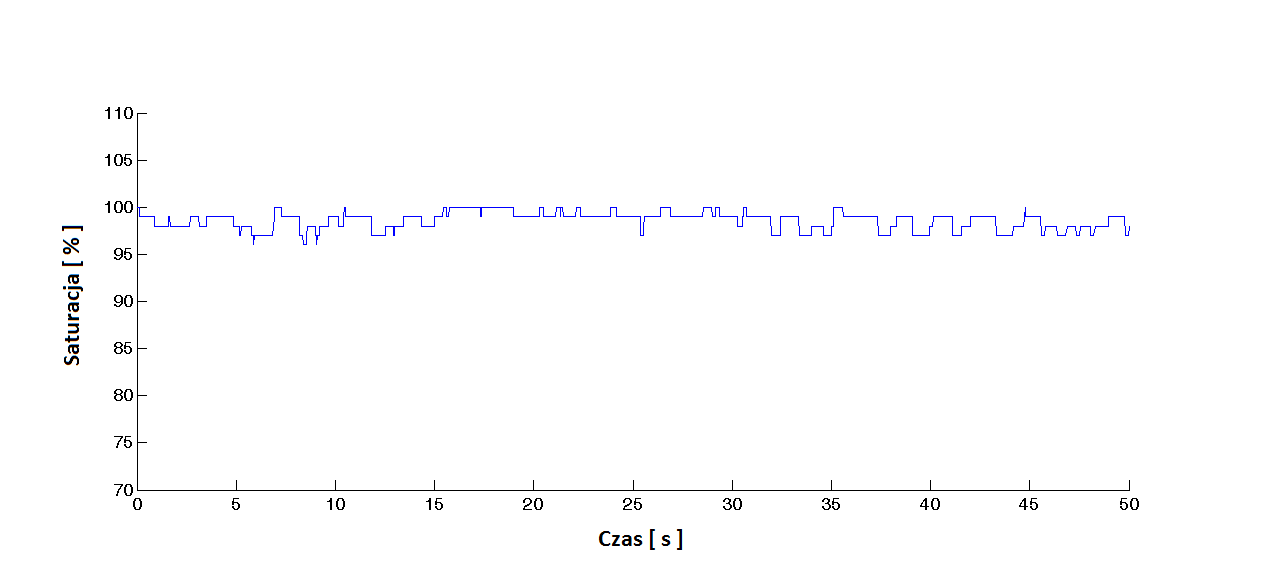
\includegraphics[scale = 0.63]{graphic/Sat30K}}
	\caption{Pomiar saturacji chwilowej - pacjent w~wieku 30 lat (kobieta)}
	\label{rys:Sat30K}
\end{figure}
\begin{figure}[!h]
	\centerline{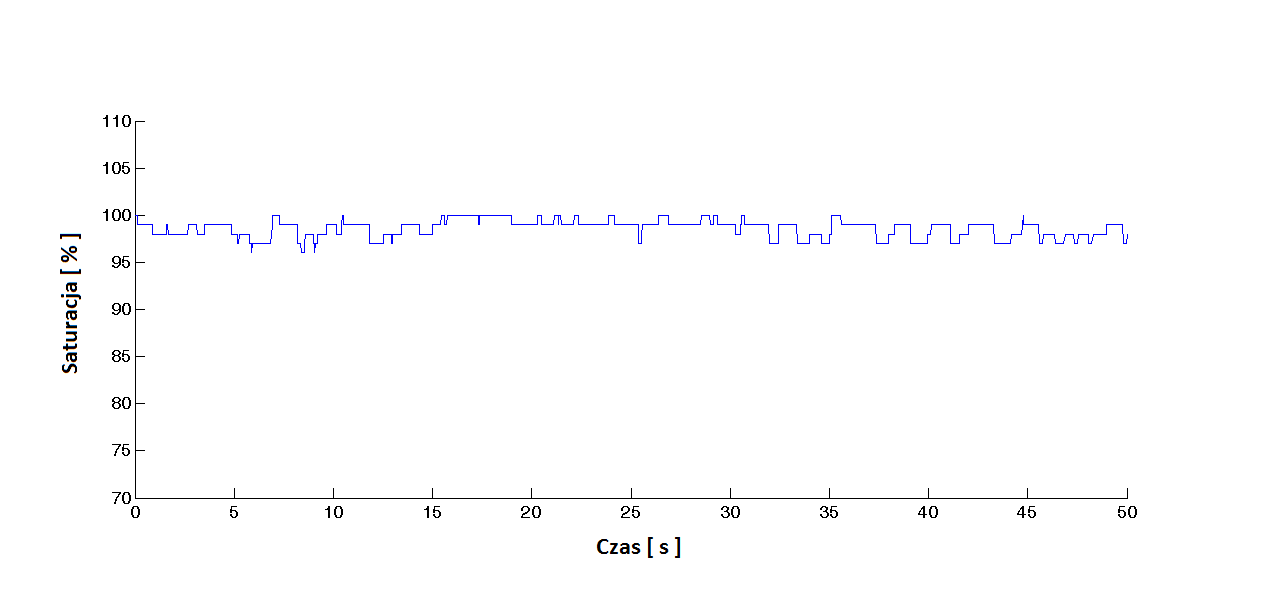
\includegraphics[scale = 0.63]{graphic/Sat30M}}
	\caption{Pomiar saturacji chwilowej - pacjent w~wieku 30 lat (mężczyzna)}
	\label{rys:Sat30M}
\end{figure}
\newpage
\begin{figure}[!h]
	\centerline{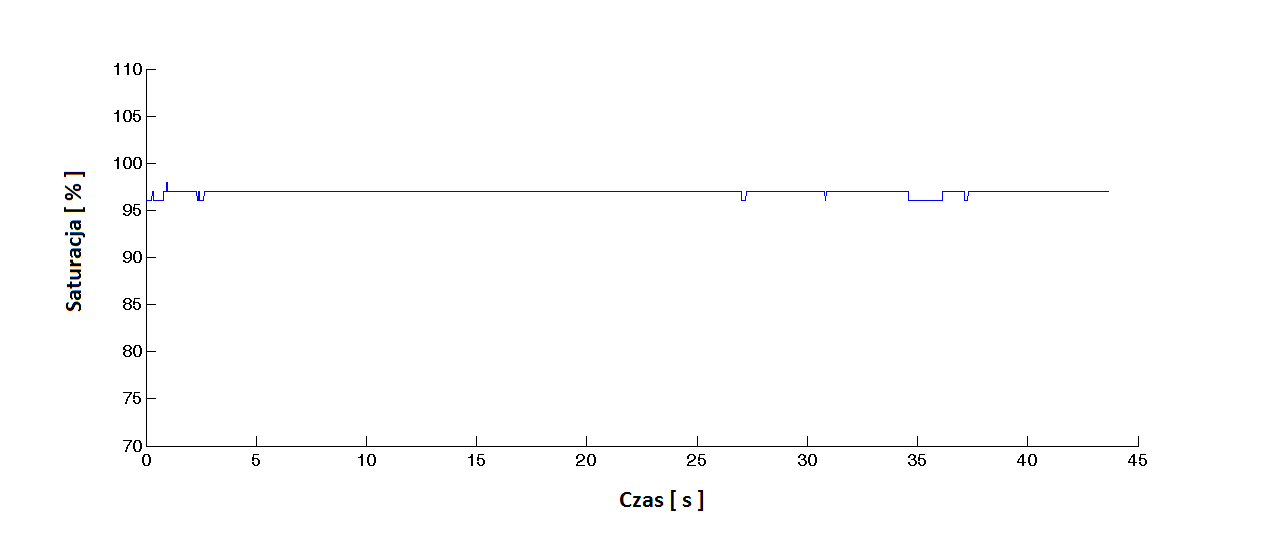
\includegraphics[scale = 0.61]{graphic/Sat50M}}
	\caption{Pomiar saturacji chwilowej - pacjent w~wieku 59 lat (mężczyna)}
	\label{rys:Sat50M}
\end{figure}
\begin{figure}[!h]
	\centerline{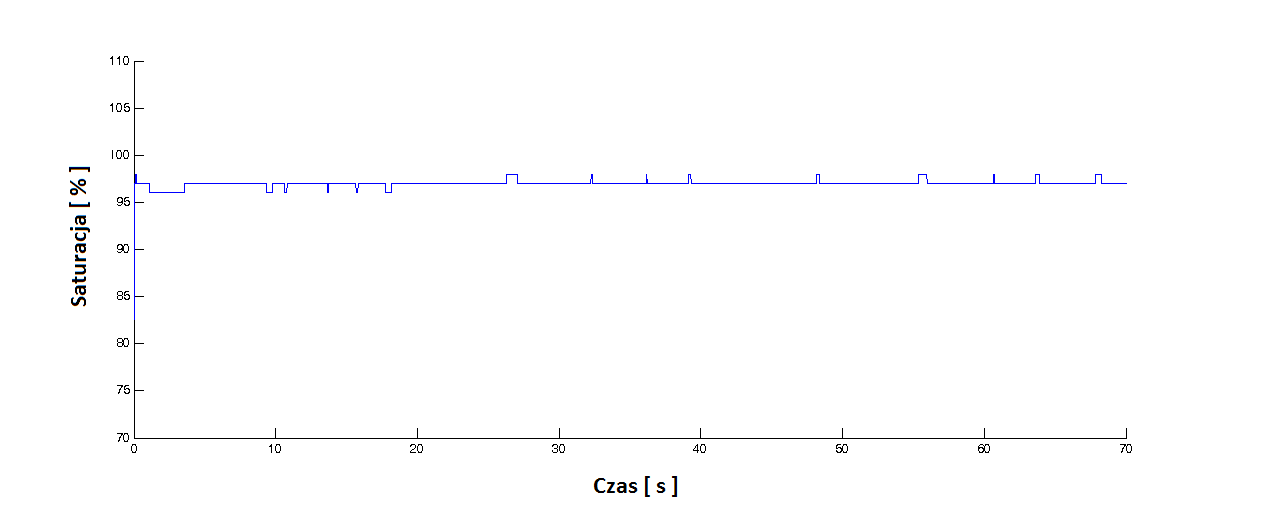
\includegraphics[scale = 0.61]{graphic/Sat90}}
	\caption{Pomiar saturacji chwilowej - pacjent w~wieku 90 lat (kobieta)}
	\label{rys:Sat90}
\end{figure}

\noindent Wyniki testów weryfikujących powtarzalność uzyskiwanych wyników przedstawia rysunek~\ref{rys:SatProba}. Spadek wartości
saturacji będący skutkiem zmniejszania dopływu tlenu do płuc zaobserwowano podczas testu polegającego na długotrwałym wstrzymywaniu
oddechu~(rys.~\ref{rys:spadek}).
\begin{figure}[!ht]
	\centerline{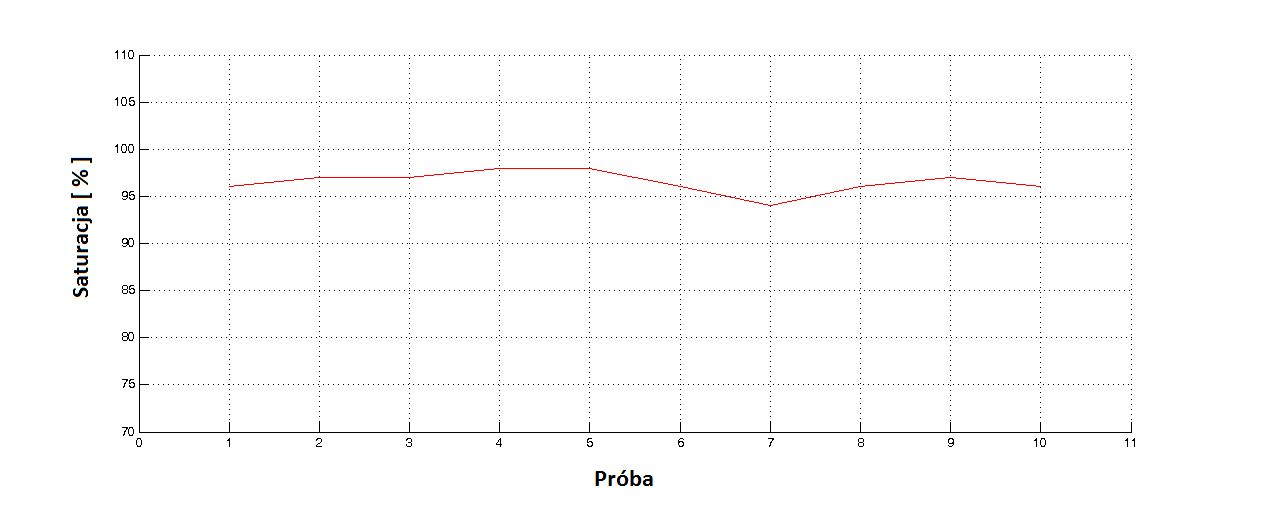
\includegraphics[scale = 0.58]{graphic/SatProba}}
	\caption{Wartość saturacji wyznaczona dla pacjenta podczas kolejnych prób pomiarowych}
	\label{rys:SatProba}
\end{figure}\\
\begin{figure}[!ht]
	\centerline{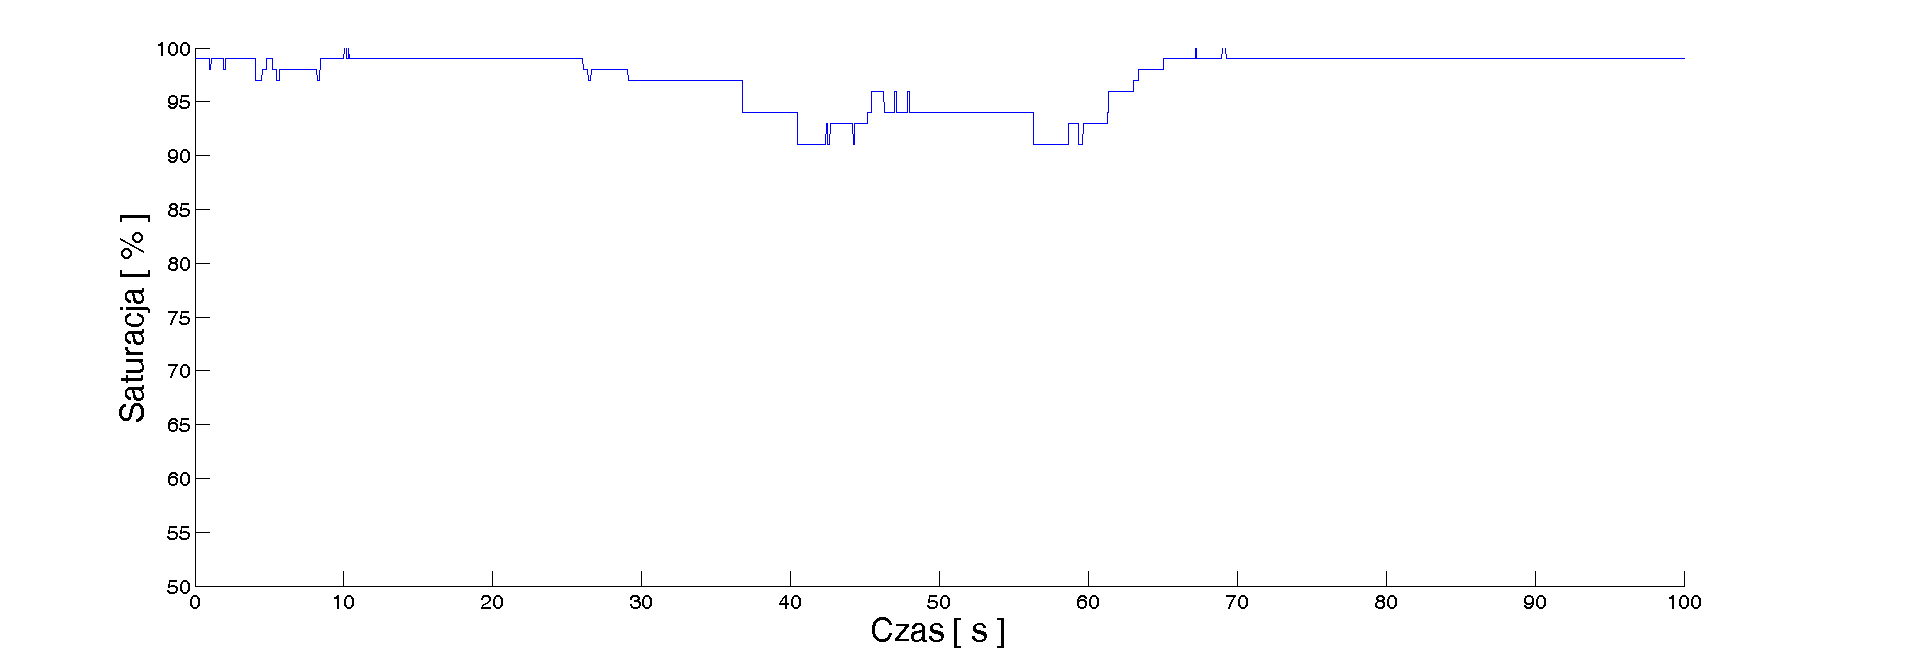
\includegraphics[scale = 0.38]{graphic/spadek}}
	\caption{Wpływ wstrzymywania oddechu na wskaźnik wysycenia krwi tętniczej tlenem}
	\label{rys:spadek}
\end{figure}\\

Pomiary saturacji krwi tętniczej wykazały brak zależności wartości wskaźnika SpO2 od wieku badanego pacjenta. Zaobserwowano
niewielki rozrzut parametru wokół wartości 96\%, która zawarta jest w~dopuszczalnym zakresie.   
\noindent Bazując na przykładowej, empirycznej krzywej kalibracyjnej dokonano serii pomiarów, których wyniki pokrywają się
z~wartościami oczekiwanymi. W~celu kompletnej kalibracji zaprojektowanego urządzenia, należy dokonać
analizy gazometrycznej krwi o~różnym stopniu wysycenia tlenem, co posłuży do określenia krzywej kalibracji konkretnego 
aparatu pomiarowego. 
